\documentclass[9pt, a4paper]{article}
\usepackage[utf8]{inputenc}
\usepackage[czech]{babel}
\usepackage[T1]{fontenc}
\usepackage{graphicx}
\usepackage{amsmath, amssymb, amsthm}
\usepackage[margin=2.5cm]{geometry}
\usepackage{url}
\usepackage{float}

\begin{document}

\begin{titlepage}
    \begin{center}
        {\large {Přírodovědecká fakulta}} \\
        \vspace{0.2cm}
        {\large Univerzita Karlova}
        
        \vspace{1.5cm}
        
\includegraphics[width=0.5\linewidth]{img/PrFUK_strom_digital_cerna.png} 
        \vfill{}
        
        {\huge\bfseries Digitální model terénu} \\
        \vspace{0.5cm}
        {\large {Algoritmy počítačové kartografie}} \\
        \vfill
        
        \begin{center}
            \large Teodor Sorokáč \\
        \end{center}
        \vfill{}

        \begin{center}
            \ 2. N-GKDPZ \\
            \ Praha 2026
        \end{center}
        
    \end{center}
\end{titlepage}

\newpage
\section{Zadání}

\vspace{5mm}
\subsection*{\textbf{Úloha č. 3: Digitální model terénu}}

\vspace{3mm}
\noindent\textit{Vstup: množina \ $P = \{ p_i, ..., p_n\}, p_i = \{x_i, y_i, z_i\}.$}
\vspace{3mm}

\noindent\textit{Výstup: polyedrický DMT nad množinou $P$ představovaný vrstevnicemi doplněný vizualizací skolnu trojúhelníků a jejich expozicí.}
\vspace{3mm}

\noindent Metodou inkrementální kontrukce vytvořte nad množinou $P$ vstupních bodů 2D Delaunay triangulaci. Jako vstupní data použijte existující geodetická data (alespoň 300 bodů) popř. navrhněte algoritmus pro generování syntetických vstupních dat představující významné terénní tvary (kupa, údolí, spočinek, hřbet, ...).
\vspace{3mm}

\noindent Vstupní množiny bodů včeteně níže uvedených výstupů vhodně vizualizujte. Grafická rozhraní realizujte s využíváním frameworku QT. Dynamické datové struktury implementujte s využitím STL. 
\vspace{3mm}

\noindent Nad takto vzniklou triangulací vygenerujte polyedrický digitální model terénu. Dále proveďte tyto analýzy:
\vspace{3mm}

\begin{itemize}
    \item S využitím lineární interpolace vygenerujte vrstevnice se \textit{zadaným krokem} a v \textit{zadaném intervalu}, proveďte jejich vizualizaci s rozlišením zvýrazněných vrstevnic.
    \item Analyzujte sklon digitálního modelu terénu, jednotlivé trojúhelníky vizualizujte v závislosti na jejich sklonu.
    \item Analyzujte expozici digitálního modelu terénu, jednotlivé trojúhelníky vizualizujte v závislosti na jejich expozici ke světové straně.
\end{itemize}
\vspace{3mm}

\noindent Zhodnoťte výsledný digitální model terénu z kartografického hlediska, zamyslete se nad slabinami algoritmu založeného na 2D Delaunay triangulaci. Ve kterých situacích (různé terénní tvary) nebude dávat vhodné výsledky? Tyto situace graficky znázorněte.
\vspace{3mm}

\noindent Zhodnocení činnosti algoritmu včetně ukázek proveďte alespoň na \textbf{3 strany} formátu A4 

\vspace{0.3cm}
\subsection*{\textbf{Hodnocení:}}

\begin{center}
\resizebox{\textwidth}{!}{
\begin{tabular}{|l|c|}
\hline
\textbf{Krok}                                                                                  & \textbf{Hodnocení} \\ [0.5ex]  \hline\hline
Delaunay triangulace, polyedrický model terénu. &  10b \\ \hline
Konstrukce vrstevnic, analýza sklonu a expozice. & 10b \\ \hline
\textit{Triangulace nekonvexní oblasti zadané polygonem.}                                              & \textit{+5b} \\ \hline
\textit{Výběr barevných stupnic při vizualizaci sklonu a expozice.}                                    & \textit{+3b} \\ \hline
\textit{Automatický popis vrstevnic.}                                                                  & \textit{+3b} \\ \hline
\textit{Automatický popis vrstevnic respektující kartografické zásady (orientace, vhodné rozložení).} & \textit{+10b} \\ \hline
\textit{Algoritmus pro automatické generování terénních tvarů (kupa, údolí, spočinek, hřbet, ...).} & \textit{+10b} \\ \hline
\textit{3D vizualizace terénu s využitím promítání.}                                                   & \textit{+10b} \\ \hline
\textit{Barevná hypsometrie.} & \textit{+5b} \\ \hline\hline
\textbf{Max celkem:} & \textbf{65b} \\ \hline
\end{tabular}}
\end{center}


\vspace{0.3 cm}
\newpage
\section{Popis a~rozbor problému}
\vspace{0.3 cm}

Digitální model terénu (DMT) slouží v geografických informačních systémech jako matematická aproximace reálného zemského povrchu v digitálním prostředí. Skládá se ze souboru prostorově lokalizovaných bodů s definovanou výškovou složkou a z interpolačního pravidla, které umožňuje rekonstruovat nadmořskou výšku modelovaného území.

\vspace{0.3 cm}

\noindent V rámci této úlohy je povrch reprezentován pomocí nepravidelné trojúhelníkové sítě TIN (Triangulated Irregular Network). Tento model představuje spojitý polyedrický povrch složený z navzájem navazujících rovinných trojúhelníků. Hlavní předností sítě TIN oproti pravidelným rastrovým strukturám je schopnost lépe zachytit rozmanitost terénu např. v oblastech s výraznými terénními tvary (jako jsou hřbety, údolnice či prudké svahy).

\subsection*{Delaunayho triangluace (DT)}
\vspace{0.3 cm}
\noindent Aby polyedrický model správně interpretoval tvar povrchu, musí být vstupní body propojeny ideálním způsobem. V počítačové kartografii se pro tento účel nejčastěji uplatňuje Delaunayova triangulace. Klíčovým prvkem je, že maximalizuje minimální vnitřní úhel ze všech možných triangulací nad danou množinou bodů. Tímto způsobem zamezuje vzniku nevhodných, úzkých trojúhelníků, které by mohly způsobovat geometrické zkreslení při analýzách.

\vspace{0.3 cm}
\noindent Základním kritériem této triangulace je podmínka prázdné kružnice. Tato podmínka tedy zajišťuje, že uvnitř kružnice opsané trojúhelníku se nesmí nacházet další bod.

\subsection*{Active Edge List (AEL)}
\vspace{0.3 cm}
\noindent Tvorba DT probíhá využitím dynamického seznamu aktivních hran – AEL (Active Edge List). Jedná se o seznam hran, které nemají přiřazený třetí bod, pro doplnění do trojúhelníku.

\vspace{0.3 cm}
\noindent Zásadním pravidlem je, že každá vnitřní hrana může být součástí pouze dvou trojúhelníků. Tímto způsobem je zajištěna čistota a jednoduchost sítě.

\vspace{0.3 cm}
\noindent Algoritmus postupně odebírá hrany ze seznamu AEL a mění jejich orientaci. Pro každou vybranou hranu hledá v její levé polorovině takový bod, který splňuje podmínku největšího minimálního úhlu. 

\vspace{0.3 cm}
\noindent Pokud je optimální bod nalezen, vytvoří se nový trojúhelník. Dvě nové hrany, které tento trojúhelník doplňují, jsou zkontrolovány vůči seznamu AEL. Pokud se v něm již nacházejí v opačné orientaci, znamená to, že sousední trojúhelník je hotov a tyto hrany se ze seznamu odstraní. Pokud se pro danou hranu v levé polorovině nepodaří nalézt žádný vhodný bod, je přímo zapsána do výsledné sítě jako finální prvek. Algoritmus takto iteruje dokud není list AEL prázdný.

\newpage
\subsection*{Konstrukce vrstevnic pomocí lineární interpolace}
\vspace{0.3 cm}
\noindent Výpočet vrstevnic v trojúhelníkové síti TIN probíhá lokálně uvnitř každého elementu. Protože je každý trojúhelník aproximován jako rovinná plocha, průsečíkem této plochy s horizontální rovinou vrstevnice je přímá úsečka.

\vspace{0.3 cm}
\noindent Proces vyhledávání průsečíků probíhá sekvenčním testováním všech hran trojúhelníku. Pro každou hranu vymezenou koncovými body $P_1 = [x_1, y_1, z_1]$ a $P_2 = [x_2, y_2, z_2]$ algoritmus nejprve ověřuje výškovou podmínku protnutí:

\vspace{0.3 cm}
$$(z - z_1)(z - z_2) < 0$$

\vspace{0.3 cm}
\noindent Pokud hrana touto podmínkou projde, znamená to, že rovina vrstevnice o výšce $z$ protíná úsečku $P_1P_2$ v jejím vnitřním bodě. Přesné horizontální souřadnice tohoto průsečíku $[x, y]$ jsou následně dopočítány na základě lineární interpolace, která předpokládá konstantní sklon terénu podél zkoumané hrany:

\vspace{0.3 cm}
$$x = \frac{x_2 - x_1}{z_2 - z_1}(z - z_1) + x_1$$
\vspace{0.3 cm}
$$y = \frac{y_2 - y_1}{z_2 - z_1}(z - z_1) + y_1$$

\vspace{0.3 cm}
\noindent Při praktické realizaci je nutné korektně ošetřit specifické (kolineární) stavy, kdy hrana leží přímo v rovině vrstevnice, což matematicky vyjadřuje rovnost:

\vspace{0.3 cm}
$$(z - z_1)(z - z_2) = 0$$

\newpage
\subsection*{Analýza sklonu terénu (slope)}
\vspace{0.3 cm}
Sklon terénu reprezentuje úhel $\phi$, který svírá rovina trojúhelníku v síti TIN s referenční rovinou. Výpočet se provádí samostatně pro každý trojúhelník sítě.

\vspace{0.3 cm}
\noindent Máme rovinu trojúhelníku určenou třemi prostorovými vrcholy $P_1=[x_1,y_1,z_1]$, $P_2=[x_2,y_2,z_2]$ a $P_3=[x_3,y_3,z_3]$. Nejprve se stanoví směrové vektory dvou jeho hran $\vec{u}$ a $\vec{v}$:

\vspace{0.3 cm}
$$\vec{u}=(x_3-x_2, \ y_3-y_2, \ z_3-z_2)$$

\vspace{0.3 cm}
$$\vec{v}=(x_1-x_2, \ y_1-y_2, \ z_1-z_2)$$

\vspace{0.3 cm}
\noindent Vektorový součin těchto hran definuje normálový vektor $\vec{n}$ k rovině zkoumaného trojúhelníku:

\vspace{0.3 cm}
$$\vec{u} \times \vec{v} = \vec{n} = (n_x, n_y, n_z)$$

\vspace{0.3 cm}
\noindent Následně se spočítá velikost (norma) tohoto normálového vektoru:

\vspace{0.3 cm}
$$\|\vec{n}\| = \sqrt{n_x^2 + n_y^2 + n_z^2}$$

\vspace{0.3 cm}
\noindent Finální sklon povrchu $\phi$ se poté odvodí z kosinu úhlu mezi normálou a svislou osou:

\vspace{0.3 cm}
$$\cos \phi = \frac{n_z}{\|\vec{n}\|}$$

\subsection{Analýza expozice terénu (aspect)}
\vspace{0.3 cm}
Expozice (neboli orientace svahu ke světovým stranám) je definována jako azimut $A$ průmětu normálového vektoru roviny trojúhelníku do referenční vodorovné roviny. Pro její výpočet se opětovně využívají složky dříve stanoveného normálového vektoru $\vec{n} = (n_x, n_y, n_z)$.

\vspace{0.3 cm}
\noindent Směr této orientace se určuje z poměru horizontálních komponent normály na základě vztahu:

\vspace{0.3 cm}
$$\tan A = \frac{n_y}{n_x}$$

\newpage
\section{Aplikace}
\vspace{0.5 cm}
Aplikace se otevře spuštěním skriptu MainForm.py a otevře se interaktivní okno, ve polygon. Nad lištou tlačítek se nachází nabídka tří možností: \textit {File}, \textit {Analysis}, \textit {View}, \textit {Clear} a \textit {Settings}. Po rozkliknutí záložky \textit {File} se nabídne možnost vložení vlastního bodového mračna z textového souboru z počítače uživatele. Tlačítko \textit {Analysis} po rozkliknutí nabídne uživateli několik možností pro analýzu. Záložka \textit {View} nabídne uživateli možnost uživateli vypnout a zapnout aktivní vrstvy (DT, Slope, Aspect, Vrstevnice). Tlačítkem \textit{Clear} se uživateli nabídnou dvě možnosti a to pro smazání výsledku analýzy \textit{Clear result} nebo smazání celého plátna \textit{Clear all}. Tlačítkem \textit{Settings} se uživateli zobrazí interaktivní okno, ve kterém jsou informace ohledně rozestupu vrstevnic a také maximální a minimální výšky. Když uživatel zadá vlastní interval vrstevnic a poté klikne na "OK", vrstevnice se překreslí na požadovaný intervel. Dále je okno doplněno o záložku \textit {Open}, které nabízí možnost vložení souboru s bodovým mračnem, nad kterým lze provést zpracované analýzy: \textit {Delaunayho triangulace, vrstevnice, Slope a Aspect}. Posledním tlačítkem \textit{Exit} se interaktivní okno aplikace zavře. 
\vspace{0.3 cm}

\noindent V případě vložené vlastního bodového mračna se velikost zobrazované \vspace{0.3 cm}

\begin{figure}[h!]
    \centering
    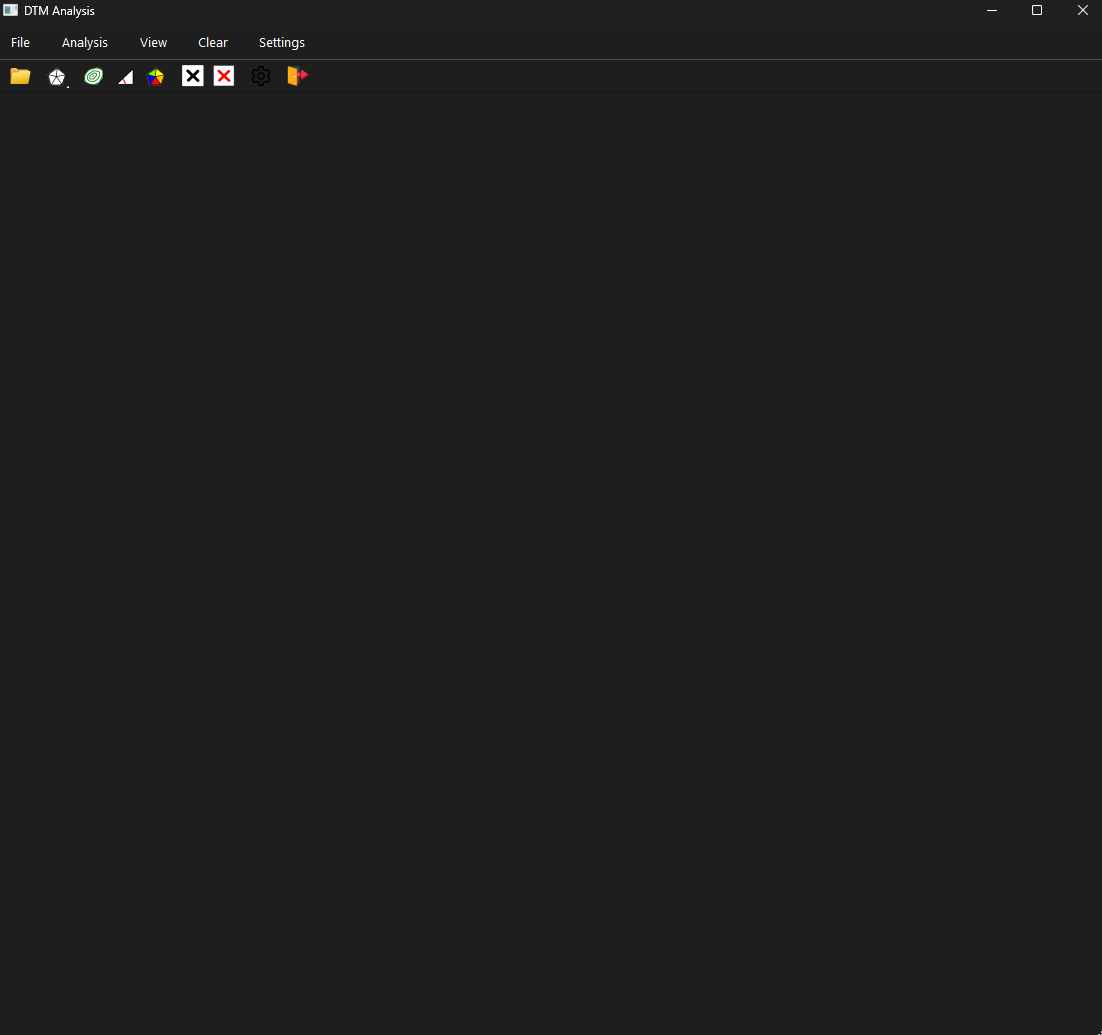
\includegraphics[width=0.5\linewidth]{img/aplikace.png}
    \caption{\centering\textit{Uživatelské prostředí aplikace}}
    \label{fig:placeholder}
\end{figure}

\newpage
\section{Dokumentace}
\vspace{0.5 cm}
Úloha byla vypracována v softwaru Visual Studio Code v jazyce Python a obsahuje několik souborů se skripty, které na sebe odkazují (algorithms.py, draw.py, MainForm.py, QPoint3DF.py, edge.py, triangle.py, settings.py). Pro zapisování skriptů byl použit formát CamelCase
\vspace{0.5 cm}

\subsection*{algorithms.py}
\vspace{0.3 cm}
V tomto souboru byly uloženy následující funkce:
\vspace{0.3 cm}

\begin{itemize}
\item \textbf{def getPointLinePosition} - Funkce matematicky vyhodnocuje vzájemnou polohu bodu a přímky pomocí determinantu.
\item \textbf{def getNearestPoint} - Funkce iterativně vyhledává a vrací prostorově nejbližší bod k zadanému referenčnímu bodu z dostupné množiny.
\item \textbf{def get2LinesAngle} - Funkce vypočítá úhel sevřený dvěma prostorovými vektory na základě jejich skalárního součinu.
\item \textbf{def findDelaunayPoint} - Funkce identifikuje optimální třetí vrchol pro vznikající trojúhelník tak, aby maximalizoval vnitřní úhel.
\item \textbf{def createDT} - Hlavní algoritmus, který nad množinou bodů generuje kompletní síť hran tvořících Delaunayovu triangulaci.
\item \textbf{def updateAEL} - Funkce zajišťuje správu aktivních hran (Active Edge List). Pokud se nová hrana již vyskytuje v opačném směru, je smazána, jinak je přidána.
\item \textbf{def getContourPoint} - Funkce využívá lineární interpolaci a vypočítá souřadnice průsečíku hrany s definovanou výškou vrstevnice.
\item \textbf{def createContourLines} - Funkce prochází trojúhelníkovou síť a na základě výškového intervalu generuje seznam hran představujících vrstevnice.
\item \textbf{def transformDTToTriangles} - Funkce pro datovou transformaci, která převádí nezávislé hrany sítě na trojúhelníky.
\item \textbf{def createContourLineSegment} - Funkce vytváří segment vrstevnice a poté jej přidá do listu. 
\item \textbf{def calculateSlope} - Pomocná funkce pro odvození sklonu terénu z normálového vektoru.
\item \textbf{def calculateAspect} - Pomocná funkce pro odvození orientace terénu.
\item \textbf{def DTMSlope} - Funkce pro iterativní přiřazení hodnoty sklonu všem vygenerovaným trojúhelníkům v rámci DTM.
\item \textbf{def DTMAspect} - Funkce plnící objekty trojúhelníků vypočtenými hodnotami jejich expozice.
\end{itemize}

\newpage
\subsection*{draw.py}
\vspace{0.3 cm}
V tomto souboru byly uloženy následující funkce:
\vspace{0.3 cm}

\begin{itemize}
\item \textbf{def loadPoints} - Funkce načítá vstupní data a provádí jejich geometrickou normalizaci.
\item \textbf{def openFile} - Funkce otevírá systémové dialogové okno pro načtení textového souboru (\textit{*.txt}).
\item \textbf{def createSlope} - Funkce zajišťuje plošné vykreslení trojúhelníkové sítě pro analýzu sklonu.
\item \textbf{def createAspect} - Funkce realizuje vykreslení trojúhelníků pro analýzu expozice. 
\item \textbf{def mousePressEvent} - Funkce zachytává interakci uživatele a umožňuje manuální klikání bodů do plátna.
\item \textbf{def paintEvent} - Hlavní překreslovací metoda, která se stará o samotnou vizualizaci grafiky na plátně.
\item \textbf{def clearRes} - Funkce maže výhradně vygenerované výsledky analýz (Delaunayovu triangulaci, sklon, expozici a vrstevnice) z paměti a následně překreslí plátno.
\item \textbf{def clearAll} - Funkce zajišťuje celkový reset plátna.
\item \textbf{clearRes} vymaže navíc i veškeré vstupní body a vynuluje indikátor načteného bodového mračna.
\item \textbf{def exit} - Funkce bezpečně a korektně ukončí instanci celé aplikace.
\item \textbf{Metody get* a set*} - Skupina metod, které zprostředkovávají bezpečnou výměnu dat mezi plátnem a uživatelským rozhraním (aktualizace a vrácení).
\end{itemize}

\subsection*{MainForm.py}
\vspace{0.3 cm}
V tomto souboru byly uloženy následující funkce:
\vspace{0.3 cm}

\begin{itemize}
\item \textbf{def createDTClick} - Funkce získává body z plátna, volá algoritmus Delaunayho triangulace a výsledek předává zpět k vykreslení.
\item \textbf{def createContourLinesClick} - Funkce inicializuje výpočet vrstevnic nad vytvořeným modelem terénu a vykreslí je do plátna.
\item \textbf{def createAnalyzeSlopeClick} - Funkce spouští plošnou analýzu sklonu a překresluje plátno s výslednými barvami.
\item \textbf{def createAnalyzeAspectClick} - Funkce spouští plošnou analýzu orientace ke světovým stranám a překresluje plátno.
\item \textbf{def createSettingsClick} - Funkce vyvolává dialogové okno (třída \texttt{Settings}) pro uživatelskou změnu minimální výšky, maximální výšky a kroku vrstevnic.
\item \textbf{Metody *Changed} - Skupina metod, které reagují na změnu stavu zaškrtávacích políček v menu \textit{View} a skrývají nebo zobrazují jednotlivé vrstvy.
\item \textbf{def openClick} - Funkce otevírá interaktní okno, ve kterém má uživatel možnost vložení vlastních dat.
\item \textbf{def clearAllClick} - Funkce zajišťuje kompletní reset celé scény a vymazání všech dat i analýz.
\item \textbf{def clearClick} - Funkce slouží k selektivnímu odstranění pouze vypočtených výsledků analýz.
\item \textbf{def exitClick} - Funkce zajišťuje bezpečné a korektní ukončení a zavření celé aplikace.
\end{itemize}

\newpage
\subsection*{Pomocné a datové třídy}
\vspace{0.3 cm}
Kromě hlavních souborů využívá aplikace další datové struktury:
\vspace{0.3 cm}

\begin{itemize}
\item \textbf{Třída QPoint3DF} - Třída rozšiřující nativní prvek o souřadnici Z (nadmořskou výšku) prostřednictvím přidané metody.
\item \textbf{Třída Edge} - Třída reprezentující topologickou hranu spojující počáteční a koncový bod, disponuje metodou pro prohození orientace a porovnání.
\item \textbf{Třída Triangle} - Třída obsahující trojici vrcholů s vlastními vlastnostmi.
\item \textbf{Třída Settings} - Oddělená třída, která otevře interaktivní okno, kde lze zjistit parametry pro generování vrstevnic.
\end{itemize}

\newpage
\section{Výsledky}
\vspace{0.5 cm}
Pro analýzu bylo vybráno bodové mračno Krkonoš z geoportálu ČUZK, které bylo následně upraveno v programu CloudCompare, kde došlo k redukci z 2151928 bodů na 150 náhodně vybraných bodů.

\begin{figure}[H]
    \centering
    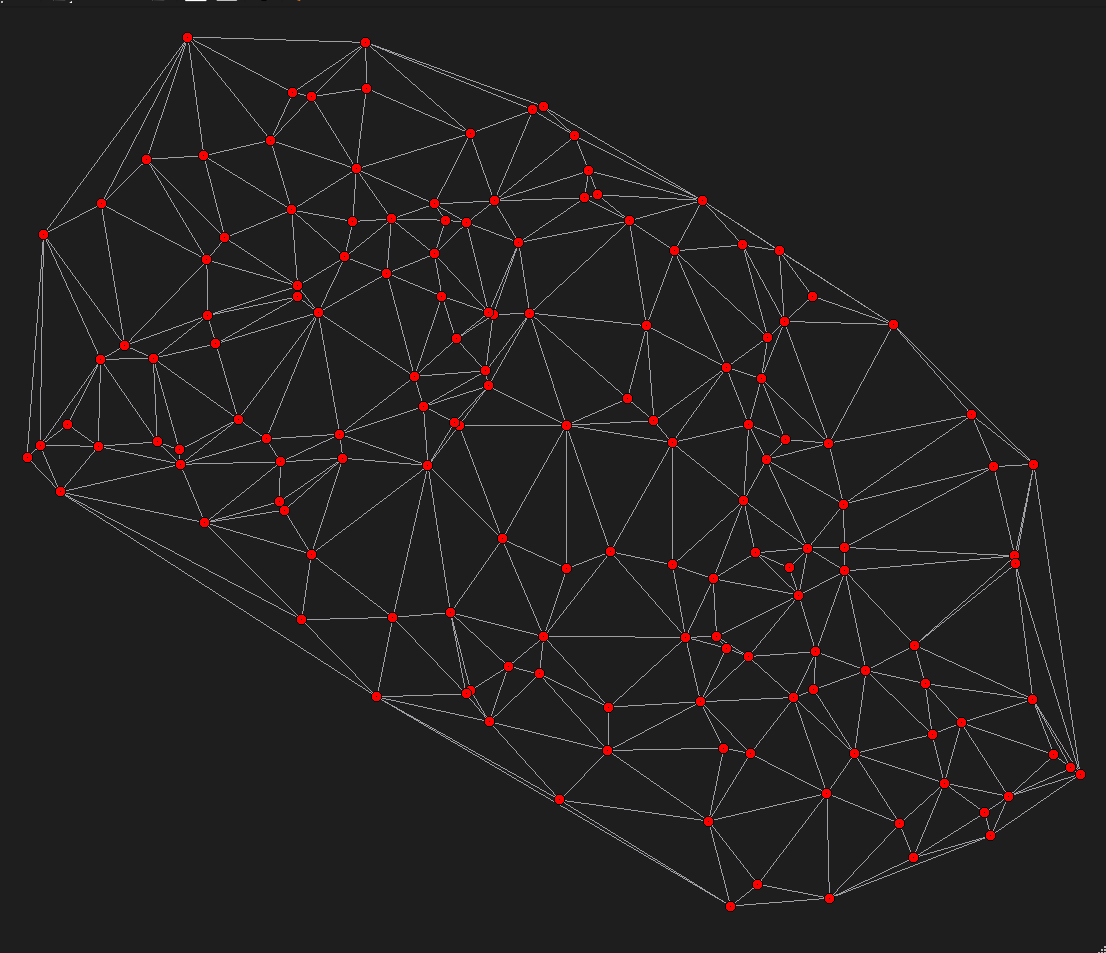
\includegraphics[width=1\linewidth]{img/DT.png}
    \caption{\centering\textit{Delaunayho triangulace}}
    \label{fig:placeholder}
\end{figure}

\noindent Na Obrázku 2. lze vidět Delaunayho triangulaci a na Obrázku 3. jsou zobrazeny vrstevnice po 25 metrech.

\begin{figure}[H]
    \centering
    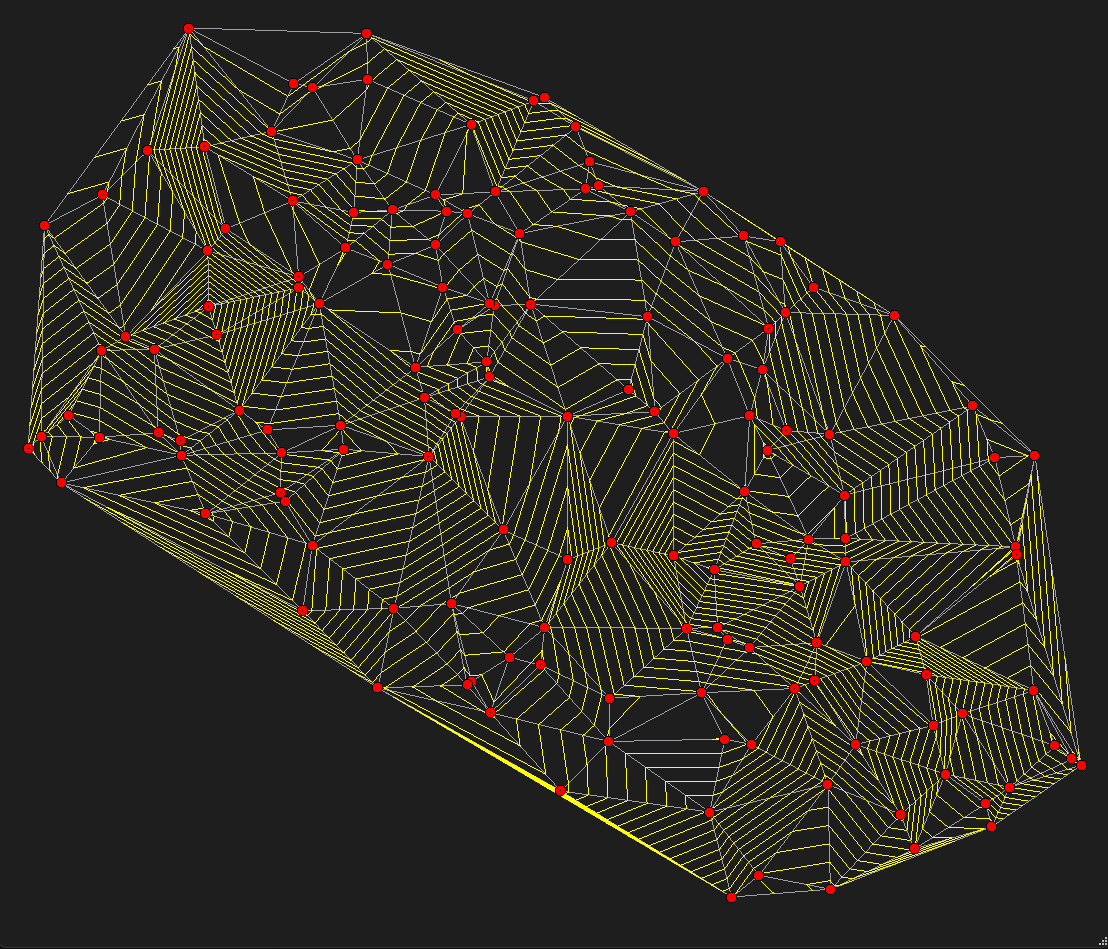
\includegraphics[width=1\linewidth]{img/vrstevnice25.png}
    \caption{\centering\textit{Vrstevnice po 25 metrech}}
    \label{fig:placeholder}
\end{figure}

\noindent Na obrázku 4. je zobrazen sklon svahů. 

\begin{figure}[H]
    \centering
    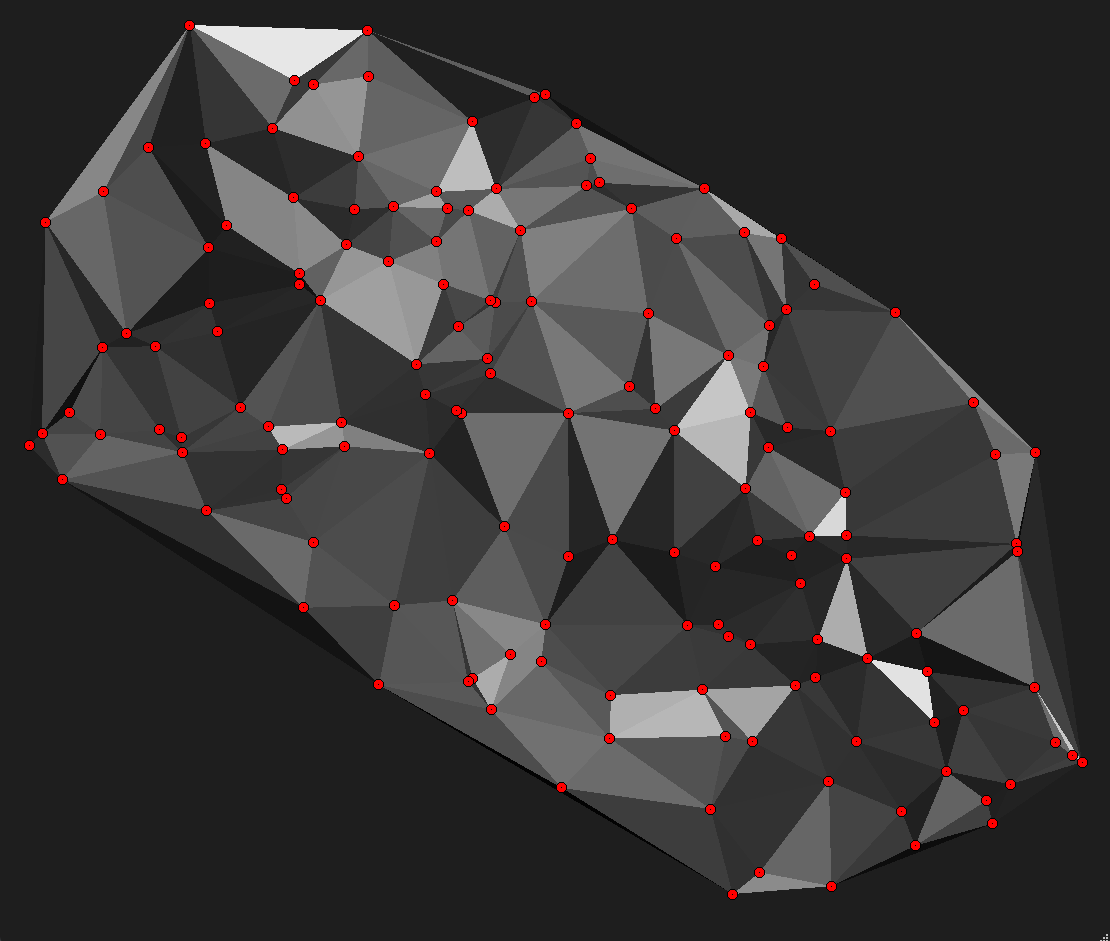
\includegraphics[width=1\linewidth]{img/slope.png}
    \caption{\centering\textit{Analýza sklonu}}
    \label{fig:placeholder}
\end{figure}

\noindent Jako poslední byla analyzována expozice svahů, která je zobrazena na obrázku 5. 

\begin{figure}[H]
    \centering
    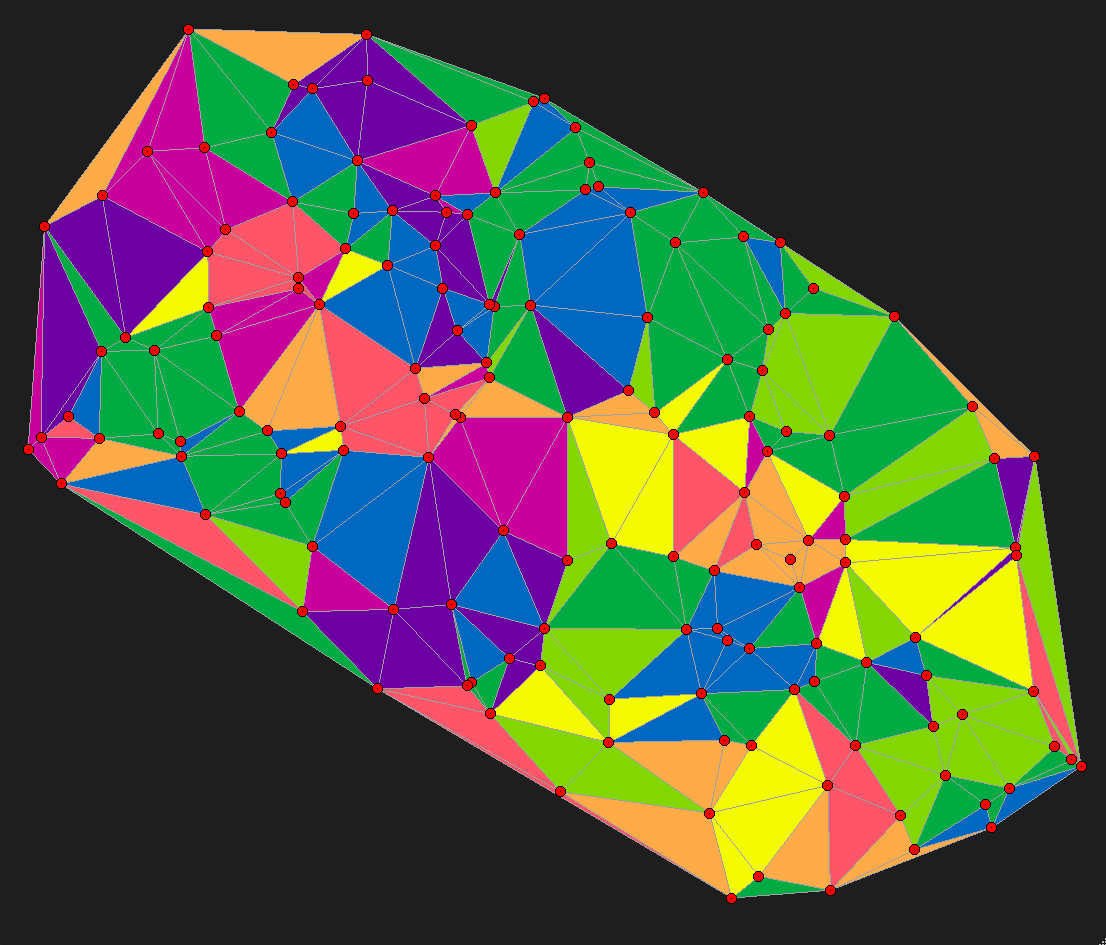
\includegraphics[width=1\linewidth]{img/aspect.png}
    \caption{\centering\textit{Analýza orientace}}
    \label{fig:placeholder}
\end{figure}

\newpage
\section{Zdroje}
BAYER, T. (2025): Rovinné triangulace a jejich využití. Greedy Triangulation. Delaunay Triangulation. Constrained Delaunay Ttriangulation. Data Dependent Triangulation. DMT. Přednáška pro~předmět Algoritmy počítačové kartografie, Katedra aplikované geoinformatiky a kartografie, Přírodovědecká fakulta UK [cit. 17.5.2025].


\end{document}